\documentclass[10pt]{article}
\usepackage{amsmath}
\usepackage{graphicx}
\usepackage{float}
\usepackage{subfig}
\usepackage{epsfig}
\usepackage{color}
%---------------------------------------------------------------------------
%
%          USER DEFINED MACROS
%
%\mathsurround = 2pt


\def \ds          {\displaystyle}
\def \rmd         {{\rm d}}
\def \be          {{\bf e}}
\def \bF          {{\bf F}}
\def \bI          {{\bf I}}
\def \bn          {{\bf n}}
\def \bff         {{\bf f}}
\def \bdf         {{\bf df}}
\def \bdT         {{\bf dT}}
\def \bT          {{\bf T}}
\def \cT          {{\cal T}}
\def \bU          {{\bf U}}
\def \bu          {{\bf u}}
\def \bv          {{\bf v}}
\def \bV          {{\bf V}}
\def \bX          {{\bf X}}
\def \by          {{\bf y}}
\def \bY          {{\bf Y}}
\def \bz          {{\bf z}}
\def \bZ          {{\bf Z}}
\def \bW          {{\bf W}}
\def \bZt         {{\bf \widetilde Z}}
\def \bzi         {{\bz}_i}
\def \bzs         {{\bz}^*}
\def \bzis        {{\bz}_i^*}
\def \bzin        {\{\bzi\}_{i=1}^k}
\def \cf          {{\cal F}}
\def \cg          {{\cal G}}
\def \ch          {{\cal H}}
\def \vi          {{V_i}}
\def \vin         {\{\vi\}_{i=1}^k}
\def \Babs        {{\Big|}}
\def \Bl          {{\Big(}}
\def \Br          {{\Big)}}
\def \Bleft       {{\Big[}}
\def \Bright      {{\Big]}}
\def \p           {\partial}
\def \R           {{\mathbb R}}
\def \N           {{\mathbb N}}
\def\y            {{\bf y}}
\def \tN          {{\widetilde{N}}}
\def \tD          {{\widetilde{D}}}

\def\m*         #1{m^{*}(\,#1\,)}
\def \proofnote #1{\footnote{{\bf Note: #1}}}
\def \norm      #1{\left|\,#1\,\right|}
\def \set       #1{\left\{\,#1\,\right\}}
\def \tr          {^T}
\def \IhH         {I_h^H}
\def \IhHb        {{\hat I}_h^H}
\def \IHh         {I_H^h}
\def \vbar        {\bar \bv}
\def \zhbar       {\bar \bz_h}
\def \zHbar       {\bar \bz_H}
\def \zhplus      {\bz_h^+}
\def \zHplus      {\bz_H^+}

\renewcommand{\theequation}{\thesection.\arabic{equation}}

\newtheorem{alg}{Algorithm}[section]
\newtheorem{thm}{Theorem}[section]
\newtheorem{lem}[thm]{Lemma}
\newtheorem{cor}[thm]{Corollary}
\newtheorem{pro}{Proposition}[section]
\newtheorem{defn}{Definition}[section]
\newtheorem{asp}{Assumption}[section]
\newtheorem{rmk}{Remark}[section]

%\def \Rblack#1{\,\hbox{R \kern-1.2em I
%    \kern.275em $^{#1}$}}
%\def \bG{{\bf G}}
%\def \bt{{\bf t}}
%\def \bzj{{\bz}_j}
%\def \bY{{\bf Y}}
%\def \byi{{\by}_i}
%\def \byj{{\by}_j}
%\def \byim{\{\byi\}_{i=1}^m}
%\def \bx{{\bf x}} 
\title{\ Progress Report until July 4th}
\author{Zichao Di}
\date{\today}
\begin{document}
  \maketitle 

\section{Linear and Bilinear Control problem}
\begin{itemize}
\item The original linear control problem has the form $\min \|y-y_{\*}\|^2+\frac{\mu}{2}\|u\|^2=f(u)$ where $y=-A^{-1}(u+f)$
\item The first exprement I tried is to apply the same idea of modifing the coarse grid bound constraint as in 1d-control so that no variable will go infeasible, but this attempt failed since 
\begin{itemize}
\item on the coarse grid, the corresponding constraint will be too limited so that variables are barely moving, then the coarse grid relaxation won't give a descent direction to fine level.
\item The second reason is this idea is not general to MG/OPT and will be very complex to the higher dimension.
\end{itemize}
\item Also, during the process, notice that the search direction is always 10 times tinier than the step to solution,and  this may imply that the scaling of original problem is an issue.
\begin{itemize}
\item The first try is to scale the original problem by $h^2$, it turns out that MG/OPT for unconstrained even failed, the reason is according to the shifted problem, our goal should be to have $\nabla f_{H}(x_{H})\approx I_{h}^{H}\nabla f_{h}(x_{h})$. If we use $\|u\|^2=h^{2}u_{h}^{T}u_{h}$, then the gradients will be $\mu h^{2}u_{h}$ and $\mu H^{2}u_{H}$. If we use $\|u\|^2=u_{h}^{T}u_{h}$, then the gradients will be$\mu u_{h}$ and $\mu u_{H}$, so $\nabla f_{H}(x_{H})\approx I_{h}^{H}\nabla f_{h}(x_{h})$.
\begin{figure}[h]
\centering
  \subfloat[$I_H^h=16 (I_h^H)^T$]
 { 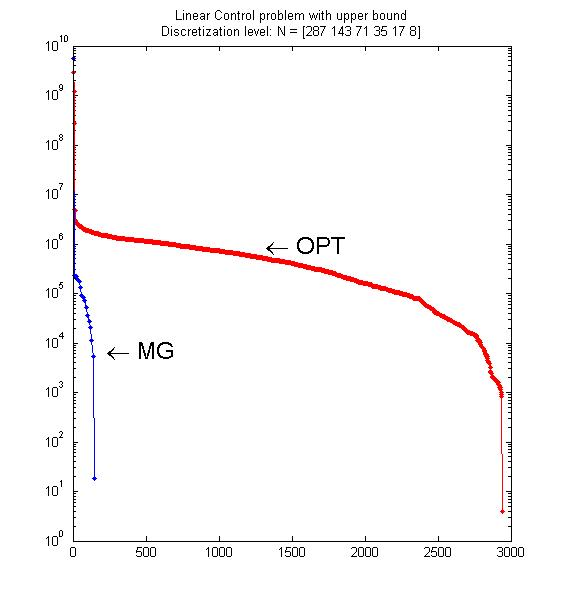
\includegraphics[width=3.3in]{goodplot287.jpg}}\\
  \subfloat[ $I_H^h=4 (I_h^H)^T$]
 { 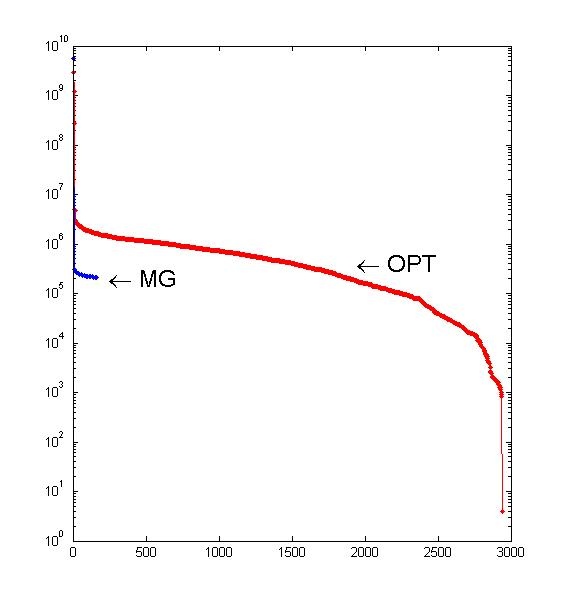
\includegraphics[width=3.3in]{badplotu287}}
  \caption{Linear control with upper bound by MG/OPT-TN }
\label{fig:good287}
\end{figure}

\item Motivated by the fact that the search direction is tiny, so I am trying enlarge the direction by multiplying the update matrix by 2, in order to keep the relation $I_H^h=c^2 (I_h^H)^{T}$, in the mean time, divide the downdate matrix by 2. And the improved result is shown in figure \ref{fig:good287}.\

i.e. Let $A=\left [ \dots \quad \frac{1}{4} \quad \frac{1}{2} \quad \frac{1}{4} \quad \dots \quad \frac{1}{2} \quad 1 \quad \frac{1}{2} \quad \dots \quad \frac{1}{4} \quad \frac{1}{2} \quad \frac{1}{4} \quad \dots \right ]$\

$I_H^h= 2A^T;  \quad I_h^H= \frac{1}{8}A$. Traditonal setting: $I_H^h= A^T;  \quad I_h^H= \frac{1}{4}A$

\begin{figure}[h]
\centering
  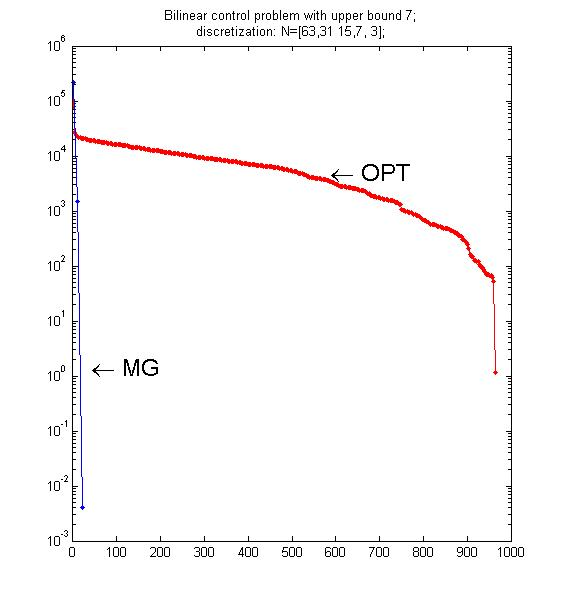
\includegraphics[width=1\textwidth]{plot63bu.jpg}
  \caption{Bilinear control problem with upper bound by MG/OPT-TN}
\label{fig:plot63bu}
\end{figure}

\item Apply the same idea of modified update and downdate matrix to the bilinear control problem by MG/OPT-TN, I got a good result too as shown in figure \ref{fig:plot63bu}.
\item Next thing I tried is to solve the same problem by fmincon first with traditional transform operators: the output is: 
\begin{quote}
\begin{verbatim}
options = optimset('Algorithm','interior-point','Display','iter', 'GradObj','on',
 'Hessian','lbfgs','MaxIter',nit, 'TolFun', 1e-8, 'InitBarrierParam',1,
'AlwaysHonorConstraints','none','InitTrustRegionRadius',63);

mesh grid is 15
J = 2.389319077691188e+006
                                            First-order      Norm of
 Iter F-count            f(x)  Feasibility   optimality         step
    0       1   2.389319e+006   0.000e+000   1.620e-002
J = 2.389319134502814e+006
    1       2   2.389319e+006   0.000e+000   2.264e-001   6.083e-002
J = 2.389319078439562e+006
    2       3   2.389319e+006   0.000e+000   2.203e-002   5.523e-002
J = 2.389319077362157e+006
    3       4   2.389319e+006   0.000e+000   1.163e-002   2.281e-003
J = 2.389319077565342e+006
J = 2.389319077565342e+006
    4       6   2.389319e+006   0.000e+000   8.475e-003   1.056e-003
J = 2.389319077470120e+006
\end{verbatim}
\end{quote}


\end{itemize}
\end{itemize} 

\section{1-D Laplacian Problem}
\begin{itemize}
\item In this problem, the best result for the fine level gradient evaluation is obtained from the modified bound constraint which different grid has its corresponding bound constraint.

\begin{figure}[h]
\centering
  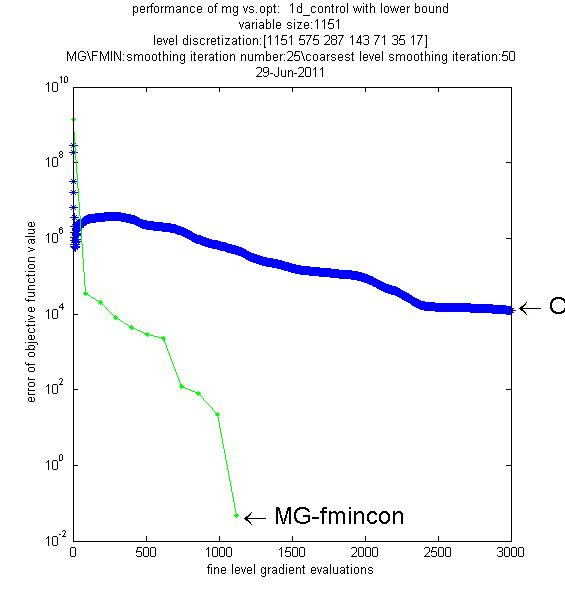
\includegraphics[width=1\textwidth]{plot1sfmin1151.jpg}
  \caption{1-D control problem with upper bound using fmincon}
\label{fig:1dcontroll}
\end{figure}

\item I also tried the same setting up of constraint using fmincon as underyling relaxation, the result is shown in figure \ref{fig:1dcontroll}, and I think the reason for fmincon working well is also that the new constraint will always keep variables feasible.

\begin{figure}[h]
\centering
  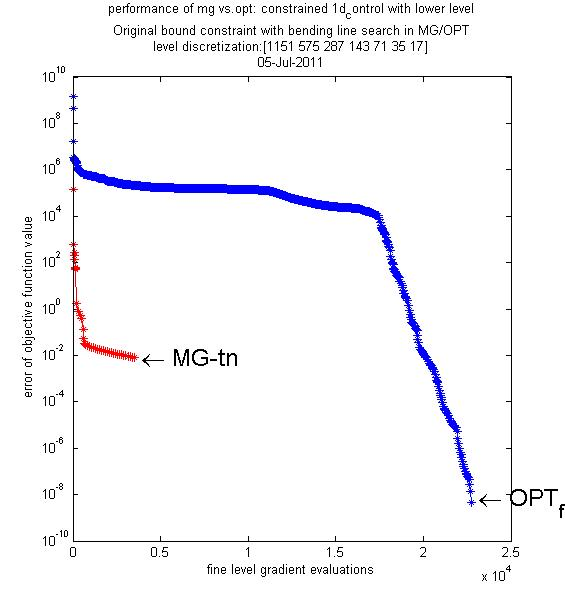
\includegraphics[width=1\textwidth]{plot1s1151bending.jpg}
  \caption{1-D control problem with lower bound using bending line search with normal constraint}
\label{fig:bending}
\end{figure}

\item The next thing I tried is using bending line search in MG/OPT with original constriant. The result is shown in figure \ref{fig:bending}. The reason for the stalling of MG/OPT is when the variable is close to solution, manually fix the infeasible point at the bounds won't decrease the merit function so that the step length is either zero or very tiny.

\end{itemize} 

\section{Next Step:}
Try to find the right scale between $I_h^H \nabla f_h (v_h)$ and $\nabla f_H (I_h^{H} v_h)$ without changing the traditional transform operator. 

\section{Interior-Point Algorithm}

The interior-point algorithm uses these options:\\

AlwaysHonorConstraint: The default 'bounds' ensures that bound constraints are satisfied at every iteration. Disable by setting to 'none'.\\

HessFcn: Function handle to a user-supplied Hessian (see Hessian). This is used when the Hessian option is set to 'user-supplied'.\\

Hessian: Chooses how fmincon calculates the Hessian (see Hessian). The choices are:

    * 'bfgs' (default)\

    * 'fin-diff-grads'\

    * 'lbfgs'\

    * {'lbfgs',Positive Integer}\

    * 'user-supplied'\\

HessMult: Handle to a user-supplied function that gives a Hessian-times-vector product (see Hessian). This is used when the Hessian option is set to 'user-supplied'.\\

InitBarrierParam: Initial barrier value, a positive scalar. Sometimes it might help to try a value above the default 0.1, especially if the objective or constraint functions are large.\\

InitTrustRegionRadius	: Initial radius of the trust region, a positive scalar. On badly scaled problems it might help to choose a value smaller than the default $\sqrt{n}$ , where n is the number of variables.\\

MaxProjCGIter	: A tolerance (stopping criterion) for the number of projected conjugate gradient iterations; this is an inner iteration, not the number of iterations of the algorithm. This positive integer has a default value of 2*(numberOfVariables - numberOfEqualities).\\

ObjectiveLimit: A tolerance (stopping criterion) that is a scalar. If the objective function value goes below ObjectiveLimit and the iterate is feasible, the iterations halt, since the problem is presumably unbounded. The default value is -1e20.\\

ScaleProblem: The default 'obj-and-constr' causes the algorithm to normalize all constraints and the objective function. Disable by setting to 'none'.\\

SubproblemAlgorithm: Determines how the iteration step is calculated. The default, 'ldl-factorization', is usually faster than 'cg' (conjugate gradient), though 'cg' might be faster for large problems with dense Hessians\\

TolProjCG: A relative tolerance (stopping criterion) for projected conjugate gradient algorithm; this is for an inner iteration, not the algorithm iteration. This positive scalar has a default of 0.01.\\

TolProjCGAbs: Absolute tolerance (stopping criterion) for projected conjugate gradient algorithm; this is for an inner iteration, not the algorithm iteration. This positive scalar has a default of 1e-10.\\




\end{document}
